%-----------------------------------------------------
% Chapter: Introduction
%-----------------------------------------------------


\chapter{Introduction}\label{chap:introduction}

Here is my awesome introduction where I use the acronym \gls{ADC}.

\section{Section}
\begin{figure}
	\centering
	\begin{subfigure}{.49\textwidth}
		\centering
		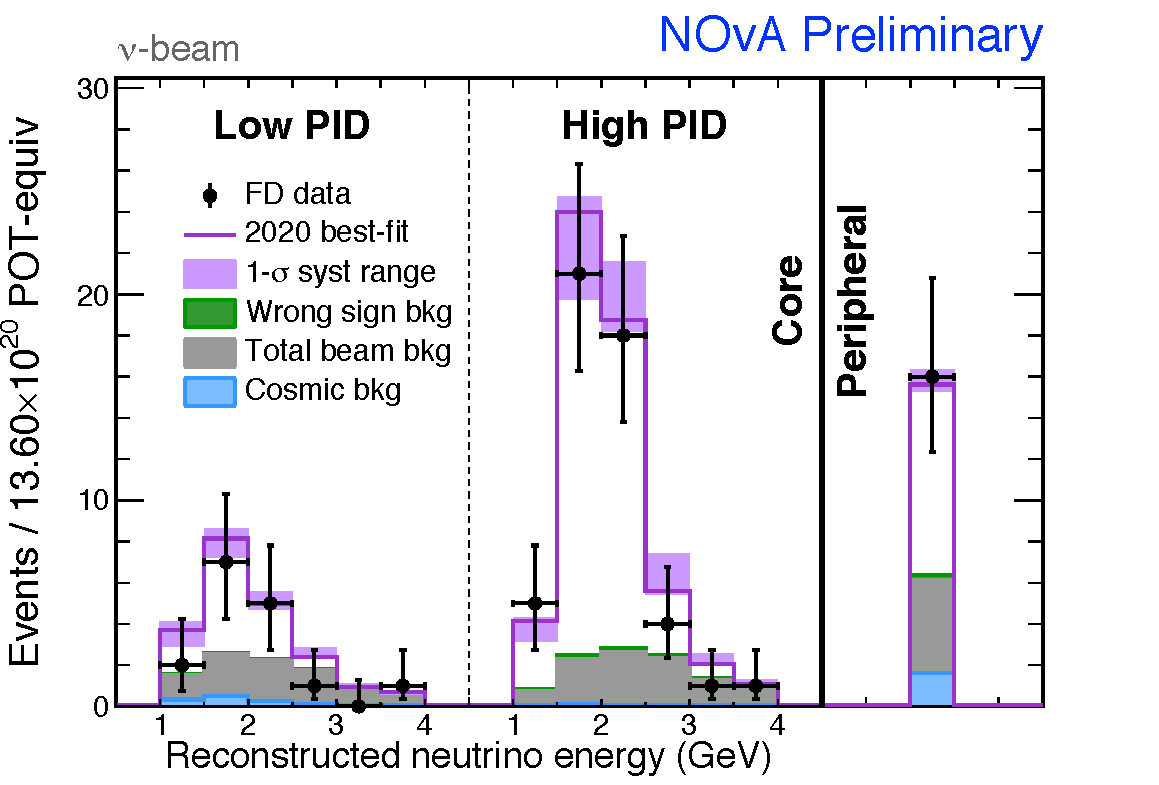
\includegraphics[width=\linewidth]{Chapter_Introduction/Plots/NOvA_NueFD_FHC.pdf}
		\caption{}
		\label{fig:nue20201}
	\end{subfigure}
	\begin{subfigure}{.49\textwidth}
		\centering
		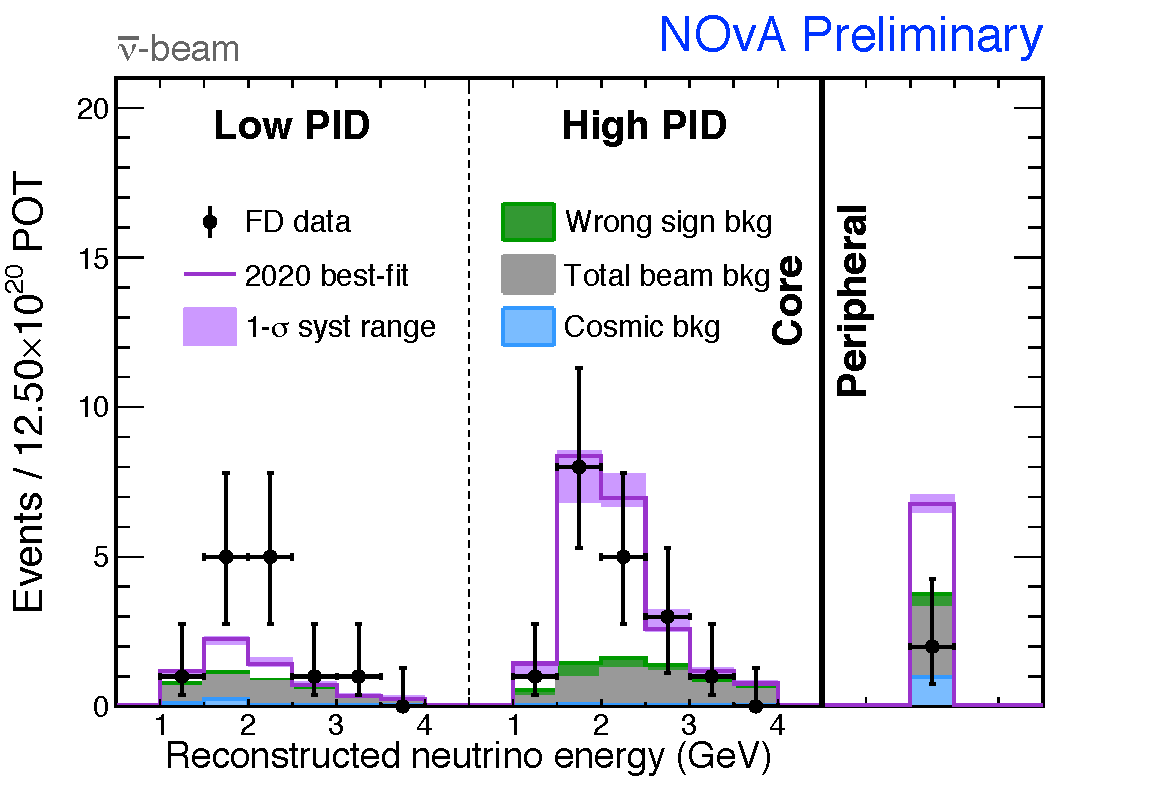
\includegraphics[width=\linewidth]{Chapter_Introduction/Plots/NOvA_NueFD_RHC.pdf}
		\caption{}
		\label{fig:nue20202}
	\end{subfigure} 
	\caption[Here is a short description of the figure.]{Here is a long description of the figure. Taken from~\cite{book:markyT}.}
	\label{fig:nue2020}
\end{figure}

\subsection{Sub-section}
\subsubsection{Sub-sub-section}

